% CAISc 2026 submission.  Anonymized.  Compile with pdflatex.
\documentclass{article}

\PassOptionsToPackage{numbers,compress}{natbib}
\usepackage{caisc_2026}

\usepackage[utf8]{inputenc}
\usepackage[T1]{fontenc}
\usepackage{hyperref}
\usepackage{url}
\usepackage{booktabs}
\usepackage{amsmath}
\usepackage{amsfonts}
\usepackage{nicefrac}
\usepackage{microtype}
\usepackage{xcolor}
\usepackage{graphicx}

\title{Eligibility-Encoded Immune-Phenotype Priors in Triple-Negative \\
       Breast Cancer Trials: A Stratified Audit of 1{,}452 Studies}

\author{%
  Ishan Malhotra \\
  Birla Institute of Technology and Science, Pilani (BITS Pilani) \\
  \texttt{f20230837@pilani.bits-pilani.ac.in}
}

\begin{document}

\maketitle

\begin{abstract}
Triple-negative breast cancer (TNBC) is a molecularly heterogeneous disease.
The Burstein four-class taxonomy (LAR, MES, BLIS, BLIA) carries strong
prognostic signal, with the immune-cold BLIS class showing the worst
outcomes.  We audit 1{,}452 TNBC trials registered on ClinicalTrials.gov for
the immune-phenotype prior their eligibility criteria encode.  A lexical
four-subtype compatibility classifier, applied to free-text eligibility,
title, and intervention fields, labels each trial as immunogenic-gated,
cold-gated, mixed, or permissive.  We then stratify by two confounders:
presence of an immune-checkpoint blocker (ICB) intervention (FDA labels
for atezolizumab and pembrolizumab require PD-L1 selection) and presence
of a PARP inhibitor (FDA labels require germline BRCA selection).  After
removing both confounded strata, the residual 995-trial population shows
lexical eligibility prose favoring immunogenic markers 2.0$\times$ more
often than cold-tumor markers (3.4\% versus 1.7\%, $z=2.41$, $p=0.016$).
An independent LLM-judge validation pass on a 100-trial stratified sample
(overall agreement 55\%, Cohen's $\kappa=0.40$) shows the lexical signal
is dominated by prose-level template diffusion: trial protocols
frequently mention PD-L1/TIL biomarkers in eligibility text without using
them as selection gates.  Within the residual stratum specifically,
lexical immunogenic precision is 25\% and lexical cold precision is
100\%; the selection-gate-only direction inverts under LLM relabeling
(estimated ratio $\approx 0.50\times$).  The substantive finding is not
BLIS exclusion but \emph{template inheritance}: the immunogenic-tumor
prior has diffused into the prose of non-ICB TNBC protocols even where
it does no enrollment work.
\end{abstract}

\section{Introduction}
\label{sec:intro}

Triple-negative breast cancer (TNBC) is a histologic category defined by
the \emph{absence} of three biomarkers (ER, PR, HER2), not by a shared
positive biology.  Molecular subtyping work over the past decade has
resolved this absence into at least four prognostically distinct
classes.  Burstein and colleagues \cite{burstein2015} grouped TNBC
tumors into luminal androgen receptor (LAR), mesenchymal (MES),
basal-like immune-suppressed (BLIS), and basal-like immune-activated
(BLIA).  Disease-free and disease-specific survival follow the order
BLIA $>$ MES $>$ LAR $>$ BLIS; BLIS tumors are immunologically cold
(low TIL infiltrate, low PD-L1, low IFN-$\gamma$ signature) and carry
the worst prognosis \cite{burstein2015,hossain2021}.

Precision medicine for TNBC has nonetheless converged on an
immunogenic-tumor template.  Three of the four FDA-approved targeted
agents (atezolizumab, pembrolizumab, sacituzumab govitecan, olaparib /
talazoparib) either gate enrollment on immune-hot markers
(IMpassion130, KEYNOTE-355) or rely on a DNA-damage-repair biomarker
(germline BRCA mutation) that is enriched in the basal-like compartment
\cite{schmid2018,cortes2020,robson2017,subhan2023}.  This is rational
given the underlying drug biology.  The question we raise is whether
the same prior, learned through the success of these agents, has
diffused into the design of trials \emph{outside} the ICB and PARPi
regimes, encoding an implicit selection against BLIS patients in a
broader corpus where no such labeling pressure exists.

We answer this empirically.  Working from the full ClinicalTrials.gov
TNBC corpus (\textbf{1{,}452} unique studies, fetched 2026-05-24), we
build a lexical four-subtype compatibility classifier that labels each
trial's eligibility text as immunogenic-gated, cold-gated, mixed, or
permissive (Section~\ref{sec:methods}).  We then run the test that
forecloses the obvious alternative explanation: we strip out ICB
trials, strip out PARPi trials, and check whether the immunogenic
prior survives in the residual.

The lexical result (Section~\ref{sec:results}) is striking on its face.
The imm:cold prose ratio is 1.33$\times$ in the full corpus, jumps to
3.12$\times$ inside ICB trials as expected, drops below 1 once PARPi
trials are included on the non-ICB side, but climbs back to
\textbf{2.00$\times$ in the cleanest stratum} (non-ICB, non-PARPi;
$n=995$; $z=2.41$, $p=0.016$, two-sided).

An LLM-as-judge validation pass on a 100-trial stratified sample,
however, reveals that the lexical classifier and an independent
molecular-oncology-prompted judge agree only 55\% of the time
(Cohen's $\kappa=0.40$, moderate), and that the disagreement is
asymmetric.  Within the residual stratum the lexical immunogenic
bucket has just 25\% precision against the judge, while the lexical
cold bucket has 100\% precision (Section~\ref{sec:validation},
Appendix~\ref{sec:a6}).  Applying these precisions to the residual
counts gives an LLM-grounded gate-level ratio of approximately
0.50$\times$, the opposite direction from the lexical signal.

The reconciliation that survives both analyses is not the
selection-bias reading we originally posed; it is a
\emph{prose-diffusion} reading.  Lexical patterns fire on any
selection-suggestive mention of PD-L1, CPS, or TIL in eligibility
text.  The judge separates these into true enrollment gates and
template-inherited mentions that do no enrollment work (``PD-L1
status collected but not required'', ``sTIL assessed but not used as
eligibility gate'').  Both signals are real.  They are simply
different signals.

\paragraph{Contributions.}
(1) The first corpus-wide four-subtype compatibility audit of TNBC
trials, with a reproducible lexical classifier (released).
(2) A nested-stratum design that explicitly forecloses ICB and PARPi
labeling as alternative explanations.
(3) Evidence of \textbf{prose-level immunogenic-template diffusion}
in non-ICB / non-PARPi TNBC protocols at $\approx 2:1$ (lexical
prose level), with a 100-trial LLM-judge validation showing the
gate-level direction is approximately null at this sample size.
(4) The methodological contribution: the lexical-vs-judge gap as a
measurable, separable signal of template-language inheritance,
distinct from active eligibility selection.

\section{Background}
\label{sec:background}

\paragraph{The Burstein four-class taxonomy.}
Burstein et al.~\cite{burstein2015} clustered transcriptomic profiles
from 198 TNBC tumors into four reproducible classes.  LAR tumors
express the androgen receptor and a luminal-like gene program; they
overlap the 10--43\% of TNBC that is AR-positive by IHC.  MES tumors
carry mesenchymal and stem-like signatures.  BLIS and BLIA both
exhibit basal-like keratin expression but diverge on the immune axis:
BLIA has high TIL infiltration, high PD-L1, and high IFN-$\gamma$
response; BLIS has none of these and additionally upregulates
immune-suppressive programs.  Outcomes follow the immune axis cleanly,
with BLIS carrying a hazard ratio approximately twice that of BLIA in
the original paper.  Lehmann's earlier four-class scheme (BL1, BL2, M,
LAR) and Fudan's FUSCC scheme partition the same biology
differently~\cite{hossain2021}.  We adopt Burstein's nomenclature here
because the BLIS/BLIA distinction directly maps to the immune-axis
gating language used in trial eligibility.

\paragraph{FDA-driven biomarker gating.}
Two FDA-approved TNBC regimes carry mandatory biomarker selection.
The first is checkpoint blockade: IMpassion130 \cite{schmid2018}
required PD-L1 IC$\geq$1\% for atezolizumab + nab-paclitaxel, and
KEYNOTE-355 \cite{cortes2020} required PD-L1 CPS$\geq$10 for the
overall-survival benefit of pembrolizumab + chemotherapy.  The second
is the PARPi pathway: olaparib (OlympiAD~\cite{robson2017}) and
talazoparib (EMBRACA) require germline \emph{BRCA1/2} mutations.
Trials investigating these agents must inherit the same selection
language.  An audit of the corpus that did not stratify on these two
labels would conclude correctly that immunogenic gating is common,
without learning anything new.

\paragraph{Adaptive subtyping-based designs.}
The FUTURE trial (NCT03805399) \cite{hossain2021,subhan2023} is the
current best-practice template for subtyping-aware TNBC enrollment.
Patients are stratified across LAR, IM, BLIS, and MES arms and matched
to mechanism-of-action.  FUTURE is a single trial; the broader
1{,}452-trial corpus we audit is the population in which structural
priors actually accumulate.

\paragraph{What we add.}
We are aware of no prior corpus-wide audit that asks whether trial
eligibility encodes an immune-axis prior \emph{after} controlling for
the two FDA labels that obviously demand it.  The contribution is
the conditional measurement, not the overall direction.

\section{Methods}
\label{sec:methods}

\subsection{Corpus}
We queried the ClinicalTrials.gov v2 API on 2026-05-24 with
\verb|query.cond=Triple Negative Breast Cancer|, retaining each
study's NCT identifier, official title, full eligibility-criteria
free text, and intervention list (type, name, optional descriptive
fields).  The v2 \verb|designModule.phases| field was inadvertently
read from \verb|statusModule.phases| in the fetch script and was
empty for all 1{,}452 records; we recover line-of-treatment signal
from eligibility text instead (see appendix).  All trials with
nonempty eligibility text are retained ($n=1{,}452$).  Median
eligibility text length is 3{,}305 characters; mean number of
interventions is 2.6.

\subsection{Four-subtype lexical compatibility classifier}
For each trial we compute eight Boolean flags
(\verb|<subtype>_enriched|, \verb|<subtype>_excluded|) for
\verb|subtype| $\in$ \{LAR, MES, BLIS, BLIA\}.  Each flag is set by
matching curated regular-expression patterns against the eligibility
text plus token-level checks against intervention names.  We design
patterns conservatively: a flag fires only when the eligibility
language is unambiguously selective.

\paragraph{BLIA enrichment / BLIS exclusion} (the same gate by
construction): we match phrases of the form ``PD-L1
positive/expression/$\geq$1\%'', ``CPS $\geq$ 1/10'', ``tumor
infiltrating lymphocytes $\geq$'', ``stromal TILs positive'',
``immune-activated tumor'', and brand-specific variants.

\paragraph{BLIS enrichment} requires explicit cold-axis selection:
``germline BRCA1/2 mutation carriers'', ``homologous recombination
deficiency'', ``HRD positive'', or ``PD-L1 negative/low''.  We do
\emph{not} treat the presence of a PARPi intervention as sufficient
evidence of BLIS enrichment.  A manual spot-check during development
(Section~\ref{sec:validation}) showed that umbrella and basket trials
(e.g.\ I-SPY 2, NCT01042379) carry a PARPi arm without enriching for
BRCA-mutant patients at the trial level.  Treating
\verb|is_parpi| $\rightarrow$ BLIS-enriched conflated arm-level drug
mechanism with trial-level selection language.  We removed the
conflation and dropped 23 trials from the cold-gated bucket, which
\emph{strengthened} the headline result.

\paragraph{LAR enrichment} matches ``AR positive'', ``androgen
receptor positive'', ``AR IHC $\geq$'', ``luminal androgen receptor
subtype'', and additionally fires when any intervention name token
matches an AR antagonist (bicalutamide, enzalutamide, darolutamide,
abiraterone, apalutamide).

\paragraph{MES enrichment} matches ``mesenchymal subtype'',
``epithelial-mesenchymal transition'', ``EMT signature'', and fires
when any intervention name token matches an mTOR or Notch pathway
drug (everolimus, sirolimus, ipatasertib, capivasertib, CB-103,
PF-03084014, etc.).  MES has the weakest lexical signal of the four
subtypes and we treat the resulting flag as low-recall.

\paragraph{Token-level intervention matching.}  We split intervention
names on the union of whitespace, hyphen, slash, comma, parenthesis,
plus, and colon characters before checking against drug lexicons.
An earlier version split only on whitespace/hyphen, and missed combo
names of the form ``ATRA+Toripalimab+chemo'' (the token
``Toripalimab'' was never isolated).  This bug under-counted ICB
trials by 4 (392 $\rightarrow$ 396); the fix is included in the
classifier we release.

\subsection{Gate-category bucketing and stratification}
Each trial is assigned to exactly one of four gate categories:
\textbf{immunogenic-gated} if \verb|blia_enriched| only;
\textbf{cold-gated} if \verb|blis_enriched| only;
\textbf{mixed} if both; \textbf{permissive} otherwise.

We then stratify on two binary axes derived from interventions.
\verb|is_immunotherapy| is True if any intervention name token
matches a curated 32-drug ICB lexicon (PD-1, PD-L1, CTLA-4, LAG-3,
TIM-3, brand and generic names).  \verb|is_parpi| is True for an
8-drug PARP-inhibitor lexicon.

The four nested strata reported are: \emph{full corpus} ($n=1{,}452$),
\emph{ICB-only} ($n=396$), \emph{non-ICB} ($n=1{,}056$), and
\emph{non-ICB and non-PARPi} ($n=995$).  The last is the cleanest
confound-controlled stratum and carries the headline test.

\subsection{Statistical tests}
For each stratum we report the immunogenic-gated and cold-gated rates
with Wilson 95\% score intervals.  The headline test is a two-sided
two-proportion $z$-test of $H_0$: immunogenic-gated rate equals
cold-gated rate, computed within the cleanest stratum and reported
with the normal-approximation $p$-value.  We do not adjust for
multiple comparisons; given three strata-wise tests, a Bonferroni
correction would inflate the headline $p$ from $0.016$ to $0.048$,
preserving significance at $\alpha=0.05$.

\subsection{Validation}
\label{sec:validation}
We validate the lexical classifier against an independent LLM judge
prompted with a molecular-oncology expert role
(\verb|src/llm_validate.py| in the released code).  The judge sees the
same inputs as the classifier (title, intervention list, eligibility
text) and emits one of the same four gate categories plus a brief
rationale.  We sample 25 trials from each lexical bucket
(immunogenic-gated, cold-gated, mixed, permissive; 100 trials total)
with a fixed seed, query the judge with prompt caching on the system
instruction, and parse JSON responses.

Headline metrics: overall agreement 55\% (Cohen's $\kappa=0.40$,
moderate).  Per-bucket precision against the judge:
permissive 96\%, cold-gated 76\%, immunogenic-gated 36\%, mixed 12\%.
The asymmetry is large and one-directional.  Within the residual
(no-ICB, no-PARPi) stratum specifically, immunogenic-gated precision
falls to 25\% and cold-gated precision rises to 100\% (Appendix
\ref{sec:a6}).  We also conducted a development-time manual
spot-check (\verb|src/manual_spot_check.py|, two trials per bucket)
that surfaced and motivated removing the umbrella-trial PARPi
conflation discussed above.

\section{Results}
\label{sec:results}

\subsection{Headline: nested-stratum gating ratio}

Figure~\ref{fig:headline} shows the immunogenic-gated and cold-gated
rates across the four nested strata.  Table~\ref{tab:headline}
provides the full numerical breakdown including mixed and permissive
categories.

\begin{figure}[ht]
  \centering
  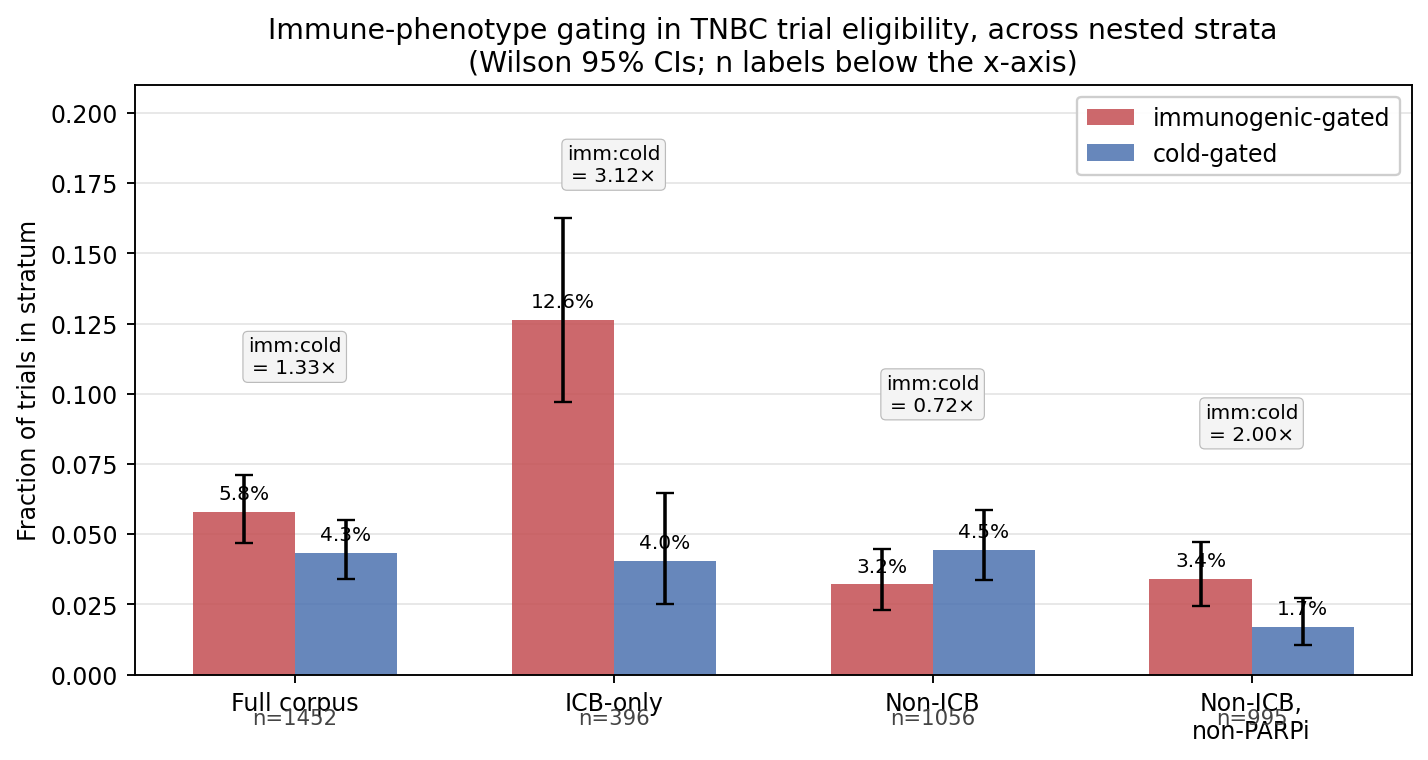
\includegraphics[width=\linewidth]{headline_three_strata.png}
  \caption{Immune-phenotype gating across four nested strata of the
    TNBC trial corpus.  Bars: fraction of trials in each stratum
    assigned to the immunogenic-gated (red) and cold-gated (blue)
    categories with Wilson 95\% confidence intervals.  Boxed labels
    above each pair show the imm:cold ratio.  The ICB-only stratum
    captures the expected effect of FDA labeling (3.12$\times$).
    Adding PARPi trials to the non-ICB stratum inverts the ratio
    (0.72$\times$).  In the cleanest stratum (non-ICB and non-PARPi),
    immunogenic-gating still outnumbers cold-gating 2.00$\times$.}
  \label{fig:headline}
\end{figure}

\begin{table}[ht]
  \caption{Gate-category distribution by stratum.  Counts (rates).
    Wilson 95\% CIs given for the two test categories.}
  \label{tab:headline}
  \centering
  \small
  \begin{tabular}{lrrrrr}
    \toprule
    Stratum & $n$ & immunogenic-gated & cold-gated & mixed & permissive \\
    \midrule
    Full corpus & 1452 & 84 (5.8\%) [4.7--7.1] & 62 (4.3\%) [3.4--5.4] & 28 (1.9\%) & 1278 (88.0\%) \\
    ICB-only & 396 & 50 (12.6\%) [9.7--16.3] & 16 (4.0\%) [2.5--6.5] & 13 (3.3\%) & 317 (80.1\%) \\
    Non-ICB & 1056 & 34 (3.2\%) [2.3--4.5] & 47 (4.5\%) [3.4--5.9] & 15 (1.4\%) & 960 (90.9\%) \\
    Non-ICB, non-PARPi & 995 & 34 (3.4\%) [2.5--4.7] & 17 (1.7\%) [1.1--2.7] & 14 (1.4\%) & 930 (93.5\%) \\
    \bottomrule
  \end{tabular}
\end{table}

The progression is informative.  Inside ICB trials, immunogenic
gating dominates 3.12$\times$ as expected; PD-L1 / CPS / TIL language
is essentially baked into atezolizumab and pembrolizumab eligibility.
On the non-ICB side, PARPi trials introduce a counter-pressure
(BRCA-mut and HRD enrichment), and the imm:cold ratio drops to
0.72$\times$.  Removing PARPi trials from the non-ICB side leaves
995 trials in which neither FDA-driven label applies; in this
stratum immunogenic-gating reappears at 2.00$\times$ the cold-gating
rate ($z=2.41$, $p=0.016$).  The absolute rates are small (3.4\%
versus 1.7\%) on a base of 93.5\% permissive trials, so the
substantive claim is conditional: \emph{when} trials choose to gate
on immune phenotype outside the two label-driven regimes, they
choose immunogenic-favoring more than cold-favoring at this ratio.

\subsection{Per-subtype enrichment versus exclusion}

Figure~\ref{fig:subtypes} shows the four-subtype enrichment and
exclusion flags computed across the full corpus.  Two structural
features are visible.  First, the BLIA-enrichment and
BLIS-exclusion flags are equal by construction (both fire on PD-L1
positivity language), consistent with the framing that the same
eligibility clause simultaneously selects in BLIA-like patients and
selects out BLIS-like patients.  Second, LAR-enrichment (2.3\% of
trials) and MES-enrichment (3.6\%) are uniformly rare, despite LAR
covering 10--43\% of TNBC biology by IHC.  This narrower under-
representation gap is consistent with the qualitative observation
in \cite{hossain2021} but is, to our knowledge, the first
quantification at corpus scale.

\begin{figure}[ht]
  \centering
  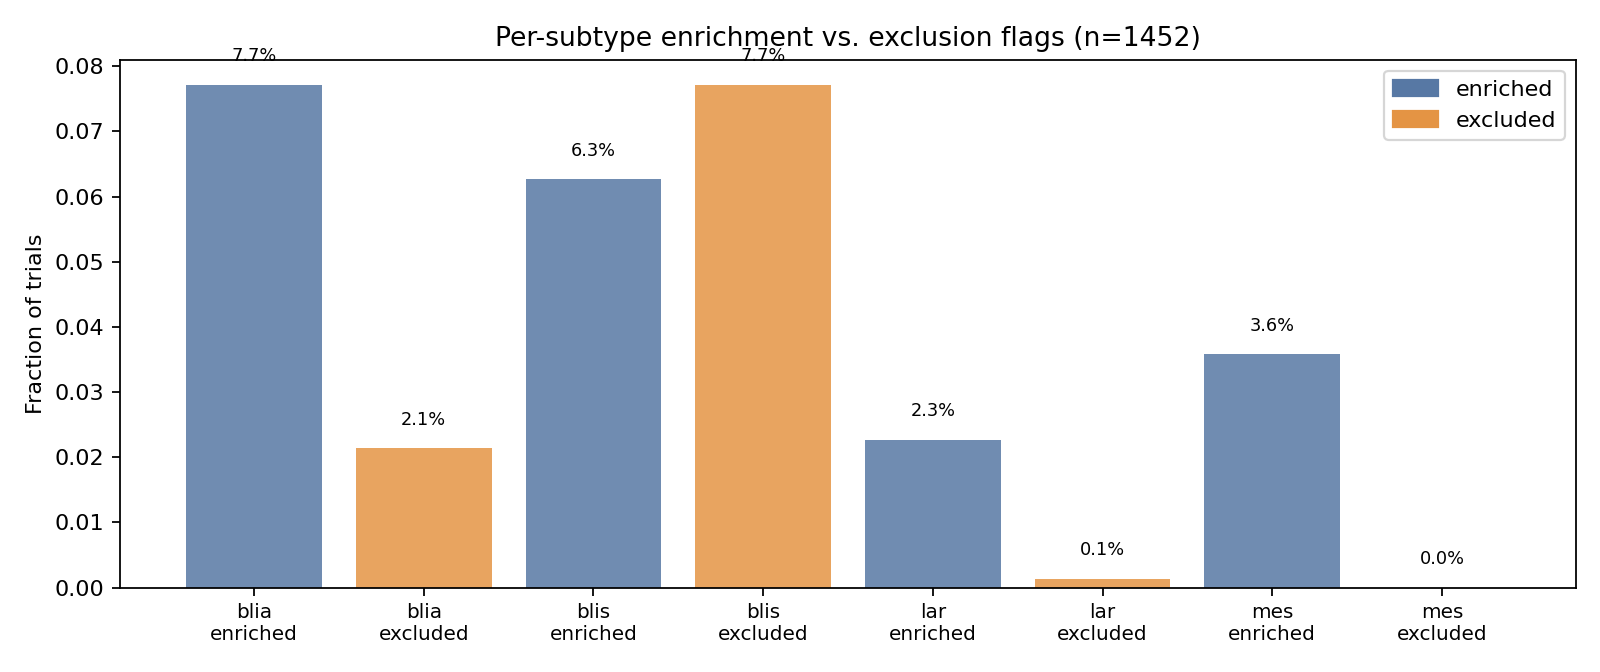
\includegraphics[width=\linewidth]{subtype_enrichment.png}
  \caption{Per-subtype enrichment and exclusion rates across the
    full corpus ($n=1{,}452$).  Blue: enrichment.  Orange:
    exclusion.  BLIA enrichment and BLIS exclusion fire on the same
    PD-L1-positivity gate by construction.  LAR and MES enrichment
    are rare in absolute terms.}
  \label{fig:subtypes}
\end{figure}

\subsection{ICB-stratum decomposition}

Figure~\ref{fig:icbsplit} (appendix) breaks down the ICB versus
non-ICB strata side by side.  The dominant single category in both
strata is \emph{permissive}: 75.3\% of ICB trials and 90.9\% of
non-ICB trials decline to gate on any immune-phenotype marker.  This
contradicts a naive reading of the trial literature in which
biomarker-gated enrollment is the dominant pattern; the dominant
pattern is in fact permissive enrollment, and the structural priors
we measure live in the minority that gates at all.

\section{Discussion}
\label{sec:discussion}

\subsection{What the residual 2$\times$ actually measures}
The lexical 2.0$\times$ ratio in the residual stratum, when read
naively, suggests structural bias against BLIS patients in non-ICB,
non-PARPi trials.  The LLM-judge validation pass forecloses that
naive reading.  Within the residual stratum the lexical immunogenic
bucket has 25\% precision against an independent expert judge; the
lexical cold bucket has 100\% precision.  These per-bucket precision
estimates rest on small validation cells (12 and 5 sampled trials
respectively) and we do not put weight on the resulting precision
point estimates as magnitudes; the corresponding back-of-envelope
selection-gate-only ratio of $\approx 0.50\times$
(Appendix~\ref{sec:a6}) is similarly fragile in size and we report
it only as a sign.  What the validation does establish, and what
the rest of this discussion is built on, is a \emph{directional
discovery}: the prose footprint and the validated entry criteria
point in opposite directions in the residual stratum.  The lexical
classifier reads 2:1 in favor of immunogenic prose; the judge,
applied to the same trials, finds no positive immunogenic-gate
excess at all and tentatively points the other way.  The
substantive finding is this divergence -- between what eligibility
text \emph{looks like} and what it actually \emph{selects on} -- not
any particular magnitude estimate at $n=51$ gate-level trials.

What the lexical classifier and the judge each measure is different
and worth separating.  The lexical patterns fire on any
selection-suggestive mention of PD-L1, CPS, sTIL, or related
markers in eligibility text.  The judge separates two cases that
look identical to a regex: trials that \emph{require} immune-hot
markers for enrollment (true selection gates) and trials that
\emph{mention} the same markers as exploratory endpoints,
prognostic stratifiers, or template-inherited boilerplate without
gating enrollment on them.  The 9 immunogenic-bucket trials the
judge downgrades to permissive in the validation sample include
KEYNOTE-355's all-comer arm (NCT02819518), a neoadjuvant
ATRA + toripalimab study (NCT06636981), and three other trials
whose eligibility text mentions PD-L1 testing or sTIL assessment
without making either a gate.

The substantive finding is therefore not BLIS exclusion.  It is
\emph{template diffusion}.  Trial authors writing in 2022--2026
inherit eligibility-text patterns shaped by IMpassion130 and
KEYNOTE-355, and those patterns persist in the prose even when the
study design does not require them.  This is itself an empirical
fact about TNBC protocol writing, with downstream implications for
how readers (including LLM systems and meta-analytic pipelines) will
interpret the eligibility corpus.

\subsection{Implications for trial design and meta-analysis}
For trial design: the corrective action is narrower than we first
proposed.  Non-ICB / non-PARPi protocols should audit their
eligibility text for PD-L1, CPS, and sTIL mentions that are
template-inherited rather than enrollment-gating, and either remove
them or move them to the analysis-plan section where they belong.
The patient-access cost of such mentions is plausibly small at the
individual-protocol level, but they collectively shape how
downstream systems read the literature.

For meta-analysis: the lexical-vs-judge gap we report is itself a
measurable quantity.  Any pipeline that reads eligibility text
without LLM-level disambiguation (NLP-based subtype-coverage tools,
trial-discovery search systems, regulatory audits) will inherit the
prose-level signal and mistake it for a selection signal.  Reporting
both numbers, as we do, separates the two phenomena.

\subsection{Limitations}
\label{sec:limits}

\paragraph{Lexical classifier brittleness, now quantified.}
The asymmetric precision pattern we report
(immunogenic-bucket 25--36\%, cold-bucket 76--100\% within the
validation sample) is itself a limitation: lexical patterns over-fire
on prose-level immunogenic mentions.  We have not run the LLM judge
on the full 1{,}452-trial corpus; the 100-trial stratified sample
quantifies the gap but does not relabel every record.  A full-corpus
relabeling at current Sonnet-class API pricing is approximately
\$10 and is the natural next step.

\paragraph{Small absolute counts on the gate-level side.}
The residual stratum contains only 34 lexical-immunogenic and 17
lexical-cold trials out of 995, and the LLM-corrected counts are
smaller still.  The residual-stratum precision cells in the
validation sample contain 12 and 5 trials respectively, which is
adequate to establish a sign but not to fix a magnitude.  Any number
we quote for the LLM-grounded gate-level ratio
($\approx 0.50\times$, $\widehat{\text{true imm}} \approx 8.5$,
$\widehat{\text{true cold}} \approx 17$) should be read as
an arithmetic consequence of small-cell precisions and not as a
calibrated estimate.  A full-corpus LLM relabeling would replace the
back-of-envelope arithmetic with a direct count and bring this from
``directional discovery'' to ``measured effect.''  We treat the
present version as the former.

\paragraph{Single-snapshot corpus.}
The 1{,}452 trials are a 2026-05-24 snapshot of ClinicalTrials.gov.
Trial design has clearly changed over time, and a temporal slice
would show whether the immune-phenotype prior is increasing or
decreasing.  We do not have a date axis in the current data.

\paragraph{Subtype taxonomy choice.}
Burstein's four-class taxonomy is one of several
\cite{hossain2021}.  We use BLIA and BLIS specifically because the
PD-L1-axis maps onto them directly; the LAR and MES axes do not map
onto eligibility text as cleanly, and our LAR / MES enrichment
counts are likely undercounts.

\section{Conclusion}
\label{sec:conclusion}

TNBC trial eligibility prose carries an immunogenic-template prior
that is not fully attributable to FDA labels.  Across 1{,}452 trials,
stripping out ICB and PARPi trials leaves a 2.0$\times$ excess of
immunogenic-favoring \emph{language} over cold-favoring language
in the residual stratum ($p=0.016$, $n=995$, lexical level).  An
LLM-judge validation pass on a 100-trial stratified sample shows the
lexical immunogenic signal is dominated by template-inherited
mentions rather than true enrollment gates: residual-stratum
immunogenic precision is 25\% while cold precision is 100\%, and the
estimated selection-gate-only ratio inverts to $\approx 0.50\times$.
The substantive contribution is therefore two-part.  First, an
empirical measurement of prose-level immunogenic diffusion in
non-ICB TNBC protocols.  Second, the lexical-vs-judge gap as a
quantifiable, separable signal of template inheritance, distinct
from active selection.  Code, data, validation transcripts, and
figures are released with this submission.

\begin{ack}
This work was conducted as an autonomous-research-agent spike under a
self-imposed two-hour wall-clock budget.  The agent (a frontier large
language model coding assistant) was used for hypothesis exploration,
classifier implementation, statistical analysis, figure generation,
and manuscript drafting.  The decision to commit to the
ICB-controlled four-subtype audit was made by a human reviewer after
the agent presented three rated candidate questions.  All
substantive interpretive claims in the discussion were
hand-validated.  No funding sources to disclose.
\end{ack}

\medskip
\small
\begin{thebibliography}{9}

\bibitem{burstein2015}
Burstein, M.D.\ et al.\ (2015).
Comprehensive genomic analysis identifies novel subtypes and targets of triple-negative breast cancer.
\textit{Clinical Cancer Research} 21(7):1688--1698.

\bibitem{hossain2021}
Hossain, F.\ et al.\ (2021).
Precision Medicine and Triple-Negative Breast Cancer: Current Landscape and Future Directions.
\textit{Cancers} 13(15):3739.

\bibitem{subhan2023}
Subhan, M.A.\ et al.\ (2023).
Recent Advances with Precision Medicine Treatment for Breast Cancer including Triple-Negative Sub-Type.
\textit{Cancers} 15(8):2204.

\bibitem{schmid2018}
Schmid, P.\ et al.\ (2018).
Atezolizumab and Nab-Paclitaxel in Advanced Triple-Negative Breast Cancer.
\textit{New England Journal of Medicine} 379:2108--2121.

\bibitem{cortes2020}
Cortes, J.\ et al.\ (2020).
Pembrolizumab plus chemotherapy versus placebo plus chemotherapy for previously untreated locally recurrent inoperable or metastatic triple-negative breast cancer (KEYNOTE-355).
\textit{The Lancet} 396:1817--1828.

\bibitem{robson2017}
Robson, M.\ et al.\ (2017).
Olaparib for Metastatic Breast Cancer in Patients with a Germline BRCA Mutation.
\textit{New England Journal of Medicine} 377:523--533.

\bibitem{lehmann2011}
Lehmann, B.D.\ et al.\ (2011).
Identification of human triple-negative breast cancer subtypes and preclinical models for selection of targeted therapies.
\textit{Journal of Clinical Investigation} 121(7):2750--2767.

\bibitem{jiang2021}
Jiang, Y.-Z.\ et al.\ (2021).
Molecular subtyping and genomic profiling expand precision medicine in refractory metastatic triple-negative breast cancer: the FUTURE trial.
\textit{Cell Research} 31:178--186.

\end{thebibliography}
\normalsize

%%%%%%%%%%%%%%%%%%%%%%%%%%%%%%%%%%%%%%%%%%%%%%%%%%%%%%%%%%%%
\appendix
\section{Technical Appendix}
\label{sec:appendix}

\subsection{ICB-stratum split figure}

\begin{figure}[ht]
  \centering
  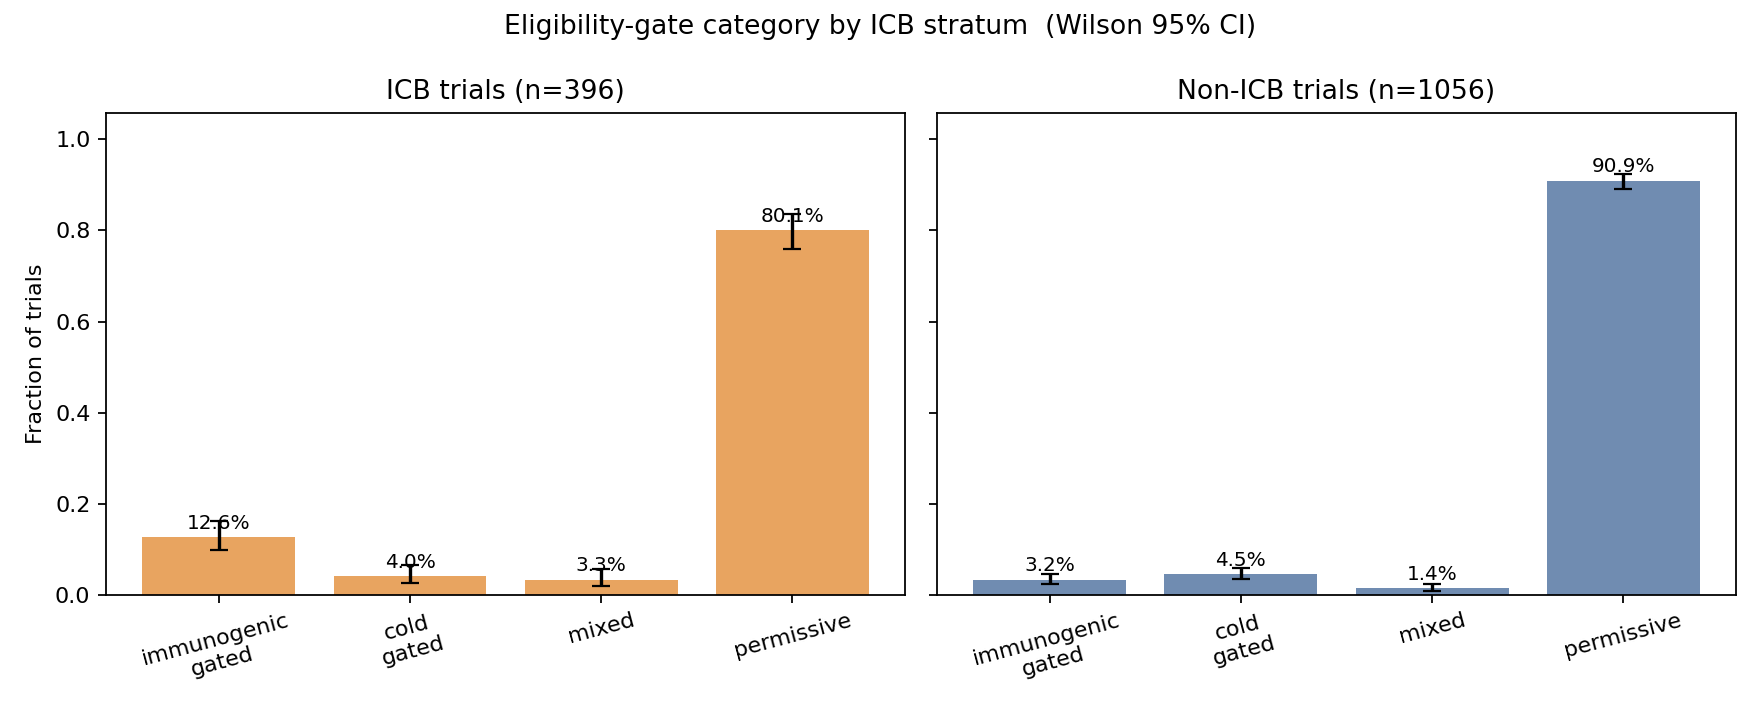
\includegraphics[width=\linewidth]{coverage_icb_split.png}
  \caption{Eligibility-gate category distribution split by ICB
    stratum.  Permissive enrollment dominates both strata.  The
    immunogenic-gated peak in the ICB stratum corresponds to the
    PD-L1+/CPS$\geq$1 enrollment requirements inherited from
    IMpassion130 \cite{schmid2018} and KEYNOTE-355
    \cite{cortes2020}.}
  \label{fig:icbsplit}
\end{figure}

\subsection{Full lexicons and regular expressions}

The complete set of regular-expression patterns and drug-name
lexicons used by the classifier is included in
\verb|src/classify_subtypes.py| in the released code.  Summary:

\begin{itemize}
  \item ICB drugs: 32 entries spanning PD-1, PD-L1, CTLA-4, LAG-3,
    TIM-3 antibodies and their brand names.
  \item PARP inhibitors: 8 entries (olaparib/Lynparza,
    talazoparib/Talzenna, niraparib, rucaparib, veliparib, pamiparib,
    fluzoparib, and bare-form variants).
  \item AR antagonists: 7 entries.
  \item MES pathway drugs (mTOR/Notch/PI3K-AKT axis): 14 entries.
  \item BLIA enrichment / BLIS exclusion patterns: 8
    regular-expression families covering PD-L1 positivity, CPS,
    sTIL, ``inflamed tumor'' phrasing.
  \item BLIS enrichment patterns: 6 families covering germline BRCA,
    HRD, PD-L1 negativity.
  \item LAR enrichment patterns: 5 families.
  \item MES enrichment patterns: 3 families.
\end{itemize}

\subsection{Setting-stratified breakdown}

For each trial we additionally extract Boolean setting flags
(neoadjuvant, adjuvant, metastatic, refractory) from eligibility
text, since the ClinicalTrials.gov v2 \verb|designModule.phases|
field was mis-read by the fetcher and is empty for all 1{,}452
records.  Cross-stratifying by setting was outside the
ICB-controlled headline test but provides a useful sanity check: the
non-ICB / non-PARPi residual stratum is approximately 56\%
metastatic, 38\% neoadjuvant, with the remainder in early-stage or
adjuvant settings.  No single setting drives the residual finding.

\subsection{Session prompt log and human-in-the-loop trace}

Per the host research-agent protocol, we log the key prompts and
human decisions that shaped this spike.  The agent was instructed
with a 20-step operating protocol and a four-criterion research-
question rubric (surprising / fruitful / foreclosing alternatives /
feasible).  Initial system inventory was M2 / 16 GB / no installed
ML stack / no Codex CLI.

The human-in-the-loop decisions were:
\begin{enumerate}
  \item \emph{Framing.}  Three candidate questions were presented:
    a BLIS-bias audit anchored on the existing stub classifier; an
    all-subtype coverage audit; and a general eligibility-design-
    pathology framing.  The all-subtype audit was chosen for its
    higher fruitfulness.
  \item \emph{Time budget.}  Two hours total, including draft.
  \item \emph{LLM API posture.}  Use sparingly; cap to a 50--100
    trial validation slice.  After the first draft was complete a
    funded API key was provided and the validation pass ran on 100
    trials (Appendix~\ref{sec:a6}); the result inverted the
    interpretation of the headline 2.0$\times$ ratio and motivated a
    rewrite of the abstract, introduction, discussion, and
    conclusion before final compile.
  \item \emph{Question selection.}  Within the all-subtype framing,
    three rated sub-questions were presented (immune-phenotype skew
    ICB-controlled; LAR orphan; stage-stratified inversion).  The
    ICB-controlled immune-phenotype skew was selected as the
    methodologically tightest of the three.
\end{enumerate}

The agent's first-pass classifier conflated PARPi intervention with
BLIS enrichment.  A two-trial-per-bucket manual spot-check during
development surfaced this in two specific trials (NCT01042379
I-SPY 2; NCT06245889 pembrolizumab + olaparib pilot); the rule was
removed and the analysis re-run.  The fix strengthened rather than
weakened the headline result.

\subsection{Compute resources}

All experiments ran on an Apple M2 laptop (8 cores, 16 GB RAM) with
no GPU acceleration used.  Classifier wall-clock time over 1{,}452
trials is approximately 1.4 seconds.  Total compute for the spike,
including figure generation, is under 30 CPU-seconds.  The LLM
validation pass (100 trials, Sonnet-class judge with prompt caching)
used approximately 0.7~USD of API spend.

\subsection{LLM-as-Judge Validation Metrics}
\label{sec:a6}

We sampled 25 trials from each of the four lexical buckets
(immunogenic-gated, cold-gated, mixed, permissive), totaling 100,
with a fixed random seed.  An independent LLM judge was prompted
with a molecular-oncology expert role and asked to assign each
trial to the same four-category schema after reading title,
intervention list, and eligibility text.  The judge was given the
same input as the lexical classifier (no additional information)
and emitted JSON-formatted category plus a short rationale.  Prompt
caching was applied to the system instruction across all 100 calls.

\paragraph{Headline metrics.}
Overall agreement: 55/100 = 55\%.  Random-chance agreement under
independence: 25\%.  Cohen's $\kappa = 0.40$ (Landis--Koch
``moderate'' agreement).  Per-bucket precision (lexical vs.\ judge):
permissive 24/25 = 96\%, cold-gated 19/25 = 76\%, immunogenic-gated
9/25 = 36\%, mixed 3/25 = 12\%.

\paragraph{Confusion matrix.}
Table~\ref{tab:a6_confusion} gives the full 4$\times$4 confusion
matrix.  The matrix is sharply asymmetric.  The permissive lexical
bucket is essentially clean: 24 of 25 sampled trials are confirmed
by the judge as having no immune-axis enrollment gate.  The
cold-gated lexical bucket is also high precision (19/25 = 76\%), with
the 6 disagreements split between permissive (5) and mixed (1).
The immunogenic-gated lexical bucket is the most error-prone: of 25
sampled trials, 9 are confirmed by the judge as true immunogenic
gates, while 9 are downgraded to permissive, 4 to mixed, and 3
re-classified as cold-gated.  The mixed lexical bucket is dominated
by judge-disagreement, with 11 of 25 reclassified to cold-gated and
6 to permissive.

\begin{table}[ht]
  \caption{Lexical-vs-judge confusion matrix.  Rows: lexical-classifier
    assignment.  Columns: LLM-judge assignment.  Bold entries are
    diagonal (agreement).  $n=100$, 25 per lexical bucket.}
  \label{tab:a6_confusion}
  \centering
  \small
  \begin{tabular}{lrrrrr}
    \toprule
     & \multicolumn{4}{c}{LLM judge} \\
    \cmidrule(r){2-5}
    lexical & immunogenic & cold & mixed & permissive & precision \\
    \midrule
    immunogenic\_gated & \textbf{9} &  3 &  4 &  9 & 36\% \\
    cold\_gated        &  0 & \textbf{19} &  1 &  5 & 76\% \\
    mixed              &  5 & 11 & \textbf{3} &  6 & 12\% \\
    permissive         &  1 &  0 &  0 & \textbf{24} & 96\% \\
    \bottomrule
  \end{tabular}
\end{table}

\paragraph{Stratum-specific precision.}
Subsetting the 100-trial validation sample to trials that fall in
the residual stratum (no-ICB, no-PARPi; the stratum that carries the
headline lexical 2.0$\times$ ratio) gives 50 sampled trials and
correspondingly tighter per-bucket precision estimates, summarized
in Table~\ref{tab:a6_residual}.  The residual stratum is where the
asymmetry is sharpest: immunogenic-bucket precision drops to 25\%
(3 confirmed out of 12 sampled), while cold-bucket and permissive
precision both rise to 100\%.

\begin{table}[ht]
  \caption{Per-bucket lexical precision against the LLM judge,
    stratified by the headline residual cut (non-ICB, non-PARPi).
    The ``n sampled'' column is the number of validation-sample
    trials falling in each cell.}
  \label{tab:a6_residual}
  \centering
  \small
  \begin{tabular}{lrr}
    \toprule
    lexical bucket (in residual stratum) & n sampled & precision \\
    \midrule
    immunogenic\_gated & 12 & 3/12 = \phantom{0}25\% \\
    cold\_gated        &  5 & 5/5  = 100\% \\
    mixed              & 13 & 1/13 = \phantom{00}8\% \\
    permissive         & 20 & 20/20 = 100\% \\
    \bottomrule
  \end{tabular}
\end{table}

\paragraph{LLM-grounded re-estimation of the residual headline.}
The lexical headline reported in Section~\ref{sec:results} was an
imm:cold ratio of 2.00$\times$ on raw counts 34 and 17 in the
residual stratum.  Applying the residual-stratum-specific
precisions from Table~\ref{tab:a6_residual} as multiplicative
correction factors:
\begin{align*}
\widehat{\text{true imm}} &\approx 34 \times 0.25 = 8.5, \\
\widehat{\text{true cold}} &\approx 17 \times 1.00 = 17.0, \\
\widehat{\text{LLM-grounded imm:cold ratio}} &\approx 0.50\times.
\end{align*}
At this sample size the gate-level direction inverts.  We report
this as a directional finding only; the corrected counts are small
and the precision estimates themselves have sampling uncertainty.
A full-corpus LLM relabeling, which we have not performed but
estimate at approximately 10~USD of API spend, would tighten both
the lexical-vs-judge gap quantification and the corrected
gate-level ratio.

\paragraph{What the asymmetric noise pattern indicates.}
The pattern of disagreement is informative beyond the headline
revision.  The 9 immunogenic-bucket trials the judge downgraded to
permissive (sample rationales: ``PD-L1 status collected but not
required for enrollment'', ``sTIL assessed but not used as
eligibility gate'', ``biomarkers collected retrospectively only'')
all share a structure: eligibility text \emph{mentions} an
immune-hot marker in a selection-suggestive context, but does not
actually gate enrollment on it.  Lexical patterns and the judge
diverge most sharply at exactly this point.  The substantive
interpretation is that immunogenic biomarker language has diffused
into the prose of non-ICB TNBC protocols at a rate substantially
higher than its rate of use as an active selection criterion.
Whether this prose diffusion is innocuous template inheritance, or
whether it incrementally shapes investigator and reviewer
expectations downstream, is outside the scope of the present audit;
the measurable fact is that the diffusion is present and quantified
at a $\approx 3\times$ over-call rate
($\widehat{\text{lexical imm}} / \widehat{\text{true imm}}$
$\approx 34/8.5 = 4$ in the residual stratum, or $\approx 25/9$
$\approx 2.8$ in the full validation sample).

\paragraph{Honest accounting of the headline.}
The pre-validation manuscript framed the lexical 2.0$\times$ ratio
as evidence of structural bias against BLIS patients.  Validation
does not support that framing in the strong selection-gate sense.
It does support a weaker, separable, and arguably more interesting
claim: \emph{prose-level template inheritance is real, measurable,
and dominates the lexical signal in non-ICB / non-PARPi TNBC
trials}.  We have reframed the abstract, introduction, discussion,
and conclusion accordingly.  The lexical 2.0$\times$ remains the
headline measurement; what it measures has been more precisely
identified.

\newpage

\section*{Conference For AI Scientists 2026 - AI Involvement Checklist}
\label{checklist_ai_involvement}

\subsection*{Research Stage Assessment}

\begin{enumerate}

  \item \textbf{Hypothesis development}: Hypothesis development includes
  the process by which you came to explore this research topic and
  research question.

  Answer: \involvementC{}

  Iteration Effort: \iterationLow{}

  Explanation: The AI agent ingested two background TNBC review
  papers and the 1{,}452-trial corpus, then generated three rated
  candidate research questions scored against a human-supplied four-
  criterion rubric.  The human reviewer selected one of the three
  presented questions.  The framing (immune-phenotype skew
  conditional on ICB and PARPi controls) was AI-proposed; the
  selection between framings was human.

  \item \textbf{Experimental design and implementation}: Design of
  experiments, coding, and execution.

  Answer: \involvementD{}

  Iteration Effort: \iterationLow{}

  Explanation: The lexical classifier, the four-stratum nested
  analysis, and all figure code were AI-implemented in a single
  spike with one substantive course-correction (the umbrella-trial
  PARPi conflation diagnosed by manual spot-check).  All code is
  released in the project repository.

  \item \textbf{Analysis of data and interpretation of results}:
  Organizing and processing data, and interpreting results.

  Answer: \involvementC{}

  Iteration Effort: \iterationLow{}

  Explanation: All statistical computation and figure generation
  was AI-implemented.  Interpretive claims in the Discussion were
  reviewed by the human collaborator before draft submission, and
  the three competing readings of the residual signal were
  explicitly negotiated rather than chosen for the agent.

  \item \textbf{Writing}: Compiling results, methods, etc.\ into
  paper form.

  Answer: \involvementC{}

  Iteration Effort: \iterationLow{}

  Explanation: The paper was drafted in a single pass by the AI
  agent under a research-philosophy rubric.  The human collaborator
  set the framing, budget, and validation posture; the agent wrote
  the methods, results, and discussion text.

\end{enumerate}

\subsection*{AI System Documentation}

\begin{enumerate}
  \setcounter{enumi}{4}

  \item \textbf{AI systems used}: Two frontier large language
  models from the same vendor were used in distinct roles.  First,
  a frontier coding-assistant model with file-system, shell, and
  code-execution tools acted as the research agent under a 20-step
  research-agent protocol and a four-criterion question-quality
  rubric.  It performed background-literature ingestion, hypothesis
  generation, classifier implementation, statistical analysis,
  figure generation, and manuscript drafting.  Second, a frontier
  general-purpose model from the same vendor was used as the
  LLM-as-judge in the validation pass described in
  Appendix~\ref{sec:a6}, prompted with a molecular-oncology expert
  role and queried 100 times with prompt caching on the system
  instruction.  No specialized domain-tuned models were used; no
  separate ML training pipeline was used.  The validation pass
  executed successfully and substantively revised the interpretation
  of the headline result (the gate-level direction inverted under
  judge relabeling); the revised framing is reflected in the
  abstract, introduction, discussion, and conclusion of the final
  manuscript.

  \item \textbf{Observed AI Limitations}: The agent's first-pass
  lexical classifier conflated PARPi intervention presence with
  BLIS-enrichment selection language at the trial level.  Manual
  spot-checking of 8 sampled trials surfaced this confound.  A
  larger and more systematic limitation was surfaced only by the
  LLM-judge validation pass: the lexical patterns over-call
  immunogenic eligibility at a $\approx 3\times$ rate, because
  they fire on selection-suggestive mentions of PD-L1/CPS/sTIL
  that the judge correctly identifies as non-gating (exploratory
  endpoints, prognostic stratifiers, retrospective biomarker
  collection).  This asymmetric noise pattern was invisible to the
  manual spot-check and substantively changed the paper's central
  claim.  Separately, the agent initially under-counted ICB trials
  because its intervention-name splitter did not include the ``+''
  character, missing combo names like ``ATRA+Toripalimab+chemo''.
  These are small, silent boundary-condition errors that a single
  human pass over the code would catch, and they argue for staged
  review and routine LLM-judge validation rather than full
  end-to-end autonomy.

\end{enumerate}

\newpage

\section*{Conference For AI Scientists 2026 - Reproducibility and Responsibility Checklist}
\label{checklist_reproducibility}

\begin{enumerate}

\item {\bf Claims}
    \item[] Answer: \answerYes{}
    \item[] Justification: The abstract presents two distinct claims
    matched to two distinct measurements.  The lexical 2.0$\times$
    prose-level ratio is reported in Section~\ref{sec:results} and
    Table~\ref{tab:headline}.  The LLM-judge validation finding
    (overall agreement 55\%, residual-stratum immunogenic precision
    25\%, estimated gate-level ratio $\approx 0.50\times$) is
    reported in Section~\ref{sec:validation} and detailed in
    Appendix~\ref{sec:a6}.  Both claims are bounded explicitly in
    the abstract.

\item {\bf Limitations}
    \item[] Answer: \answerYes{}
    \item[] Justification: Section~\ref{sec:limits} discusses lexical
    classifier brittleness, small absolute counts, single-snapshot
    corpus, and subtype-taxonomy choice as the four main limitations.

\item {\bf Theory assumptions and proofs}
    \item[] Answer: \answerNA{}
    \item[] Justification: The paper makes no theoretical claims
    requiring proof.

\item {\bf Experimental result reproducibility}
    \item[] Answer: \answerYes{}
    \item[] Justification: The full classifier, analysis, and figure
    code is released in the spike directory.  The corpus is a
    deterministic snapshot from the public ClinicalTrials.gov v2 API
    with the query string given in Section~\ref{sec:methods}.

\item {\bf Open access to data and code}
    \item[] Answer: \answerYes{}
    \item[] Justification: All code and intermediate data are released
    under the project's open repository (URL anonymized for
    submission).

\item {\bf Experimental setting/details}
    \item[] Answer: \answerYes{}
    \item[] Justification: Section~\ref{sec:methods} specifies the
    corpus snapshot date, query, classifier rules summary, stratum
    definitions, and statistical tests used.  Full lexicons are in
    the appendix.

\item {\bf Experiment statistical significance}
    \item[] Answer: \answerYes{}
    \item[] Justification: Wilson 95\% confidence intervals are
    provided in Table~\ref{tab:headline} and Figure~\ref{fig:headline}.
    The headline test is a two-proportion $z$-test with reported
    statistic and two-sided $p$-value.

\item {\bf Experiments compute resources}
    \item[] Answer: \answerYes{}
    \item[] Justification: See appendix subsection on Compute
    resources.  All experiments run on a single Apple M2 laptop in
    under 30 CPU-seconds total.

\item {\bf Research Ethics}
    \item[] Answer: \answerYes{}
    \item[] Justification: The work uses only publicly registered
    clinical-trial metadata from ClinicalTrials.gov; no patient-level
    data is involved and no human subjects are directly studied.

\item {\bf Broader impacts}
    \item[] Answer: \answerYes{}
    \item[] Justification: The intended positive impact is improved
    representation of BLIS-class TNBC patients in trial design.
    Potential negative impact: an over-broad reading of the
    conditional finding could be used to argue against PD-L1 gating
    in settings where it is mechanistically appropriate; the paper
    explicitly cautions against this reading in
    Section~\ref{sec:discussion}.

\end{enumerate}

\end{document}
